%for search with vim and okular
\synctex=1


%%=====================================================================================
% Settings
%%=====================================================================================
\newcommand{\mypapersize}{A4}
\newcommand{\mylaterality}{twoside} %% "oneside" or "twoside"
\newcommand{\myparskip}{half}
\newcommand{\myfontsize}{10pt}
\newcommand{\mylinespread}{singlespacing} % e.g.onehalfspacing, doublespacing, singlespacing
\newcommand{\mylanguage}{french} %american

\documentclass[%
  fontsize=\myfontsize,
	paper=\mypapersize,
	parskip=\myparskip,
	DIV=calc,
	headinclude=true,
	footinclude=true,
	open=right,
	appendixprefix=true,	% include appendix?
	bibliography=totoc,		% include an unnumbered unit of bibliography to the table of contents
	BCOR=10mm,        	  % binding correction (depends on how you bind
	\mylaterality,        % alternative: twoside
  \mylanguage
]{scrbook}

%Encoding
\usepackage[utf8]{inputenc}
\usepackage[T1]{fontenc}

\usepackage{float}

% language adaptions
\usepackage[\mylanguage]{babel}

%% general metadata:
\newcommand{\myauthor}{Manon Racine}  %% also used for PDF metadata (hyperref)
\newcommand{\mydocumentsubject}{Projet d'approfondissement}
\newcommand{\mysubject}{AI-enhanced LoRa Based Indoor Localization System}  %% also used for PDF metadata (hyperref)
\newcommand{\myshortsubject}{AI-enhanced LoRa Based Indoor Localization System}  %% also used for PDF metadata (hyperref)
%%\newcommand{\mykeywords}{Pedestrian detection, Deep learning, CNN, BonsEyes, Thermal images}  %% also used for PDF metadata (hyperref)

%% this information is used only for generating the title page:
\newcommand{\myuniversity}{HES-SO Master} %% your university/school
\newcommand{\myfaculty}{HE-Arc} %% your university/school

\newcommand{\mysupervisora}{Dr. Nuria Pazos}
%%\newcommand{\mysupervisorb}{Florian Sauser}

%%\newcommand{\myexpert}{Adrien Birbaumer}
%%=====================================================================================
% Colors
%%=====================================================================================
% includes some colors
\usepackage[table,usenames,dvipsnames]{xcolor}
\usepackage{color, colortbl}


% Define some colors used in the template
\definecolor{grey}{gray}{0.95}
\definecolor{dkgreen}{rgb}{0,0.6,0}

\definecolor{mauve}{rgb}{0.58,0,0.82}
\definecolor{red}{rgb}{1,0,0}
\definecolor{DispositionColor}{RGB}{0, 0, 0}


\definecolor{Red200}{HTML}{EF9A9A}
\definecolor{Red300}{HTML}{E57373}
\definecolor{Red500}{HTML}{ F44336}
\definecolor{Red800}{HTML}{ C62828}

\definecolor{Orange800}{HTML}{ EF6C00}

\definecolor{Teal900}{HTML}{004D40}
\definecolor{Teal800}{HTML}{00695C}
\definecolor{Teal200}{HTML}{80CBC4}


\definecolor{Cyan200}{HTML}{80DEEA}
\definecolor{Cyan800}{HTML}{ 00838F}

\definecolor{Blue900}{HTML}{0D47A1}
\definecolor{Blue800}{HTML}{1565C0}
\definecolor{Blue700}{HTML}{1976D2}
\definecolor{Blue600}{HTML}{1E88E5}
\definecolor{Blue500}{HTML}{2196F3}
\definecolor{Blue400}{HTML}{42A5F5}
\definecolor{Blue300}{HTML}{64B5F6}
\definecolor{Blue200}{HTML}{90CAF9}
\definecolor{Blue100}{HTML}{BBDEFB}

\definecolor{Green900}{HTML}{1B5E20}
\definecolor{Green800}{HTML}{2E7D32}

\definecolor{Grey100}{HTML}{F5F5F5}



%%=====================================================================================
%% includes pictures --> possible to include them in header/footer
%%=====================================================================================
\usepackage[pdftex]{graphicx}


%%=====================================================================================
%% Style
%%=====================================================================================
% override some list packages that they use babel -> see koma script doc
\usepackage{scrhack}

% nicer quotes
\usepackage[%
  autostyle,          % adapts language setting
  strict,             % turns warnings into errors
  english=american    % use american quotes style
]{csquotes}

\usepackage[automark]{scrpage2}							% allows usage of header and footer
\usepackage[perpage, hang]{footmisc} 				% footnote options

\renewcommand{\headfont}{\normalfont\sffamily\color{DispositionColor}}
\renewcommand{\pnumfont}{\normalfont\sffamily\color{DispositionColor}}
\addtokomafont{disposition}{\color{DispositionColor}}
\addtokomafont{caption}{\color{DispositionColor}\footnotesize}
\addtokomafont{captionlabel}{\color{DispositionColor}}

\usepackage{calc} %% used for calculation of header footer etc. ...

%% change page layout
\addtolength{\oddsidemargin}{-.875in}
\addtolength{\evensidemargin}{-.875in}
\addtolength{\textwidth}{1.75in}
\addtolength{\topmargin}{-.875in}
\addtolength{\textheight}{3in}  %1.75

% header and footer
\pagestyle{scrheadings}							% for customization for header and footer
\renewcommand{\chapterpagestyle}{scrheadings}	% include header and footer on chapter pages
\clearscrheadfoot

% http://ctan.uib.no/macros/latex/contrib/koma-script/doc/scrguien.pdf
% page 204
\ihead{\myshortsubject}
\ohead{Public}
\ifoot{\vspace{-0.25cm}\myauthor}
\ofoot{ \vspace{-0.25cm} \thepage}
\automark{chapter}
\setheadsepline[ \textwidth + 5pt ]{1pt} % seperation line for header...
\setfootsepline[ \textwidth + 5pt ]{1pt} % ... and footer
\setkomafont{footsepline}{\color{red}} 	 % change colors of seperation lines
\setkomafont{headsepline}{\color{red}}

%%=====================================================================================
%% Table on Contents
%%=====================================================================================
\setcounter{tocdepth}{2}
\setcounter{secnumdepth}{2} % change la profondeur de numérotation

\usepackage{makecell}

\usepackage{tabulary}
\newcolumntype{K}[1]{>{\centering\arraybackslash}p{#1}}

\usepackage{verbatim}


%%=====================================================================================
%% bibliography with biber/biblatex
%%=====================================================================================
\usepackage[backend=bibtex, %% using "biber" to compile references (instead of "biblatex")
            style=numeric, %% see biblatex documentation
            style=alphabetic, %% see biblatex documentation
            backref=true, %% create backlings from references to citations
            natbib=true, %% offering natbib-compatible commands
            hyperref=true,
            sorting=none, %% using hyperref-package references
]{biblatex}

%\addbibresource{../bib/bibliography.bib}
\addbibresource{bib/bibliography.bib}
%\addbibresource{bib/bibliography_VAL.bib}

%%=====================================================================================
%% SIUNITSX -- simplified usage of SI-units
%%=====================================================================================
%\usepackage[
%            group-digits=false,
%            exponent-product = \cdot, % use \cdot instead * for exponent product
%            binary-units=true,
%            load-configurations=binary,
%            load-configurations=abbreviations,
%]{siunitx}

% Easy typesetting hex and bin and oct
\usepackage[autolanguage, nosepfour]{numprint}
\usepackage{nbaseprt}

%%=====================================================================================
%% ifthen and todonotes puts to-do-notes in the printed document if you want
%%=====================================================================================
%% used to disable todonotes package
\usepackage{ifthen}
\newboolean{myaddlistoftodos}
\newboolean{showconfidential}

\reversemarginpar %To display the todo in the right margin
\setlength{\marginparwidth}{2cm} %To correct the bad placement

\usepackage[english]{todonotes}

%%=====================================================================================
%% Tables, figures, enums, etc...
%%=====================================================================================
%% nice rule's for tables try \toprule \midrule \bottomrule
\usepackage{booktabs}

%% set width of table and more
\usepackage{tabularx}										% creates tables

%% rotate tables and figures
\usepackage{rotating}

%% define caption style
\addtokomafont{caption}{\small} 	% small captions
\usepackage[font=small, width=0.9\textwidth, format=plain, labelfont=bf]{caption}

%%
\usepackage{subfigure}
\usepackage{placeins}

%% customize item look
\usepackage{enumitem}

%%=====================================================================================
%% some utility stuff
%%=====================================================================================
% improved typographical settings
\usepackage[%
    protrusion=true, %
    factor=900       %
]{microtype}

%% switch of extra space after punctuation
\frenchspacing

%% switches to Palatino with small caps and old style figures
\usepackage[%
            sc,%
            osf,%
]{mathpazo}

%% kills space between items
\setlist{noitemsep}

%doc% For additional special characters available by \verb#\ding{}#
\usepackage{pifont}  %% Sonderzeichen fuer Titelseite \ding{}

%doc% This package is required for intelligent spacing after commands
\usepackage{xspace}

%doc% This package offers strikethrough command \verb+\sout{foobar}+.
\usepackage[normalem]{ulem}

%% prevent club & widow penalty
\clubpenalty10000
\widowpenalty10000
\displaywidowpenalty10000

%% Titlepage
\usepackage{tcolorbox}


%%=====================================================================================
%% lslistening: used to include source code
%%=====================================================================================
\usepackage{listings}				% include source code

\lstset{% 							% options for representation of source code
  backgroundcolor=\color{grey},   % choose the background color; you must add \usepackage{color} or \usepackage{xcolor}
  basicstyle=\footnotesize,        % the size of the fonts that are used for the code
  breakatwhitespace=false,         % sets if automatic breaks should only happen at whitespace
  breaklines=true,                 % sets automatic line breaking
  captionpos=b,                    % ses the caption-position to bottom
  commentstyle=\color{dkgreen}, % comment style
  deletekeywords={...},            % if you want to delete keywords from the given language
  escapeinside={\%*}{*)},          % if you want to add LaTeX within your code
  frame=lines,                     % adds a frame around the code
  keepspaces=true,                 % keeps spaces in text, useful for keeping indentation of code (possibly needs columns=flexible)
  keywordstyle=\color{blue},       % keyword style
  language=C,                      % the language of the code
  morekeywords={*,...},            % if you want to add more keywords to the set
  numbers=left,                    % where to put the line-numbers; possible values are (none, left, right)
  numbersep=8pt,                   % how far the line-numbers are from the code
  numberstyle=\tiny\color{gray},   % the style that is used for the line-numbers
  rulecolor=\color{black},         % if not set, the frame-color may be changed on line-breaks within not-black text (e.g. comments (green here))
  showspaces=false,                % show spaces everywhere adding particular underscores; it overrides 'showstringspaces'
  showstringspaces=false,          % underline spaces within strings only
  showtabs=false,                  % show tabs within strings adding particular underscores
  stepnumber=1,                    % the step between two line-numbers. If it's 1, each line will be numbered
  stringstyle=\color{blue},        % string literal style
  tabsize=2,                       % sets default tabsize to 2 spaces
  title=\lstname,                  % show the filename of files included with \lstinputlisting; also try caption instead of title
}

%theme for C
\lstdefinestyle{C}{
	language=c, showspaces=false,
	keywordstyle=		\color{blue}\scriptsize,
	commentstyle=	  \color{dkgreen}\scriptsize\sffamily,
	stringstyle=		\color{mauve}\scriptsize,
	title=\lstname,
	escapeinside={//(*}{*)},
	morekeywords={},
	numbers = left, numberstyle=\tiny\color{black}
}

\usepackage{setspace} 
\usepackage{blindtext}
\usepackage{graphicx}
\usepackage[export]{adjustbox}

\usepackage[top=2.5cm, bottom=3cm, left=2.5cm, right=2cm]{geometry}

%%=====================================================================================
%% pdfcompresslevel from 0 to 10; std is fine
%%=====================================================================================
\pdfcompresslevel=9

%%=====================================================================================
%% Hyperref should always be the last package added --
%%=====================================================================================
\usepackage{hyperref}								% should be the last package to be inlcuded!

%\usepackage[%							% enables typesettings for hyperlinks
%pdftitle={\mysubject},%
%pdfauthor = {\myauthor},%
%pdfsubject = {\mysubject},%
%colorlinks={false},
%pdfcreator={pdfTex},%
%pdfkeywords={\mykeywords},%
%pdftex = true,%
%backref,%
%pagebackref=false, % creates backward references too
%bookmarks=True, %
%bookmarksopen=false, % when starting with AcrobatReader, the Bookmarkcolumn is opened
%pdfpagemode=UseOutlines,% None, UseOutlines, UseThumbs, FullScreen
%plainpages=false % correct, if pdflatex complains: ``destination with same identifier already exists''
%]{hyperref}								% should be the last package to be inlcuded!

%---------------------------------------------------------------------------------------------------
% include figures
%---------------------------------------------------------------------------------------------------
\newcommand{\myfigsrc}[5]{
\begin{figure}[htp]
	\begin{center}
		\includegraphics[width=#2\textwidth]{figures/#1}
		\captionsource{#3}{#4}
		\label{#5} %% NOTE: always label *after* caption!
	\end{center}
\end{figure}
}

\newcommand{\myfig}[4]{
\begin{figure}[htp]
	\begin{center}
		\includegraphics[width=#2\textwidth]{figures/#1}
		\caption[#3]{#3}
		\label{#4} %% NOTE: always label *after* caption!
	\end{center}
\end{figure}
}

\newcommand{\mypdfsrc}[6]{
\begin{figure}[htp]
	\begin{center}
		\includegraphics[page=#6, width=#2\textwidth, frame]{figures/#1}
		\captionsource{#3}{#4}
		\label{#5} %% NOTE: always label *after* caption!
	\end{center}
\end{figure}
}


\newcommand*{\captionsource}[2]{%
\caption[{#1}]{%
	#1%
	\\\hspace{\linewidth}%
	\textbf{Source:} #2%
}%
}



%% ========================================================================
%%  TODO: Enable/Disable
%% ========================================================================
\setboolean{myaddlistoftodos}{false}  %% "true" or "false"
%% If set to "true": the current list of open todos is added after the
%% table of contents. If \mytodonotesoptions is set to "disable", no
%% list of todos is added, independent of this setting here.


%----------------------------------------------------------------------------------------
%	\begin{document}
%----------------------------------------------------------------------------------------
\begin{document}

\frontmatter

\begin{titlepage}
	
	% MSE + HES-SO Images
	\vspace{-1cm}
	\begin{minipage}{0.49\textwidth}
		\begin{flushleft} \large
			
\includegraphics[width=0.8\textwidth]{figures/titlepage_fig/mse.pdf}
		\end{flushleft}
	\end{minipage}
	\begin{minipage}{0.5\textwidth}
		\begin{flushright} \large
			
\includegraphics[width=0.6\textwidth]{figures/titlepage_fig/hesso2.pdf}
		\end{flushright}
	\end{minipage}
	
	% HES-SO Master postal address
	\begin{flushleft}
		\footnotesize 		
		Master of Science HES-SO in Engineering\\
		Av. de Provence 6\\CH-1007 Lausanne
	\end{flushleft}
	
	% Vertical space under HES-SO Master postal address
	\vspace{1.7cm}
	
	\begin{flushright}
		{\huge Master of Science HES-SO in Engineering}
		
		\vspace{0.5cm}
		{\Large Orientation : Technologies de l’information et de la communication (TIC)}
		
		\vspace{1.7cm}

		\begin{spacing}{2.0}
			{\Huge \mysubject}
		\end{spacing}

		\vspace{1cm}
		\begin{spacing}{2.0}	
			Fait par\\
			{\huge \myauthor}
		\end{spacing}
	
		
		\vspace{1cm}
		\begin{spacing}{1.5}
			Sous la direction de\\
			{\Large \mysupervisora }\\ 
			%{\Large \mysupervisorb }
		\end{spacing}
	
		{\Large \myfaculty}

%		\begin{spacing}{1.5}
%			Expert externe\\
%			{\Large \myexpert }
%		\end{spacing}
		
		\vspace{1cm}%% Date
		{\large St-Imier, HE-Arc, \today}
	\end{flushright}
	% Bottom of the page
\end{titlepage}
\cleardoublepage
%\chapter*{Soumission du projet}
Accepté par la HES-SO//Master (Suisse, Lausanne) sur proposition de

\vspace{0.5cm}
Dr. Nuria Paszos conseillère de travail de Master

\vspace{2cm}
St-Imier, le 18.09.2018

\vspace{1.5cm}
\begin{minipage}[t]{0.5\textwidth}
	\raggedright
	Dr. Nuria Pazos\\
	Conseillère
\end{minipage}%
\begin{minipage}[t]{0.45\textwidth}
%	\raggedleft
	Prof. Didier Rizzotti\\
	Responsable de la filière MRU-TIC
\end{minipage}




\cleardoublepage

%----------------------------------------------------------------------------------------
%	Abstract
%----------------------------------------------------------------------------------------
%\chapter{Résumé}
Ce document présente une analyse de sécurité axée sur le bus CAN d'un véhicule autonome conçu par la société Navya.

Les premiers chapitres décrivent une analyse de l'état de l'art des moyens de communication utilisés dans les véhicules, qu'ils soient autonomes ou à conduite manuelle, puis se focalisent ensuite sur les communications employant le bus CAN, en expliquant les problèmes de sécurité qui peuvent être rencontrés en se basant sur les concepts généraux du chiffrement des télécommunications. 

Cette analyse explore ensuite l'architecture d'un véhicule autonome et la problématique en cas d'accès physique au bus CAN qui n'est pas protégé nativement contre les intrusions et attaques diverses.

Ensuite, des mesures physiques sur le bus CAN contrôlant la direction du véhicule démontrent effectivement la transmission en clair des informations, sans vérification de l'intégrité.

Pour terminer, différentes solutions applicables sont présentées, ainsi qu'une proposition de surcouche pour un bus CAN permettant de garantir l'intégrité et l'authentification des données transférées.
disposition de la documentation nécessaire.

{\let\clearpage\relax\par \chapter{Abstract}}
Dafuq is that report ?
%\chapter{Remerciements}
Merci Jackie
%\chapter*{Déclaration}

\noindent Je, soussigné, \myauthor, déclare sur l’honneur que le travail rendu, intitulé \enquote{\mysubject} est le fruit d’un travail personnel. Je certifie ne pas avoir eu recours au plagiat ou à toutes autres formes de fraudes. Toutes les sources d’information utilisées et les citations d’auteur ont été clairement mentionnées.


\vspace{2cm}

%% definition of the block tat contains date and signature
\newcommand{\mysignatureblock}[3]{%
	%% Sorry, this is a "bit" of a hack. Maybe someone knows a more elegant method?
	\begin{tabular}{llp{2em}l} 
		#1 & \hspace{4cm}        & & \hspace{4cm} \\\cline{2-2}\cline{4-4}
		&                     & & \\[-3mm]
		& {\footnotesize #2}  & & {\footnotesize #3}
	\end{tabular}
}

\mysignatureblock{St-Imier,}{Date}{Signature}



%----------------------------------------------------------------------------------------
%	List of Contents/Figures/Tables
%----------------------------------------------------------------------------------------
\tableofcontents
\listoffigures

\ifthenelse{\boolean{myaddlistoftodos}}{
  \newpage\todototoc \listoftodos          %% handy if you are using todonotes with \todo{}
}{}

%----------------------------------------------------------------------------------------
%	Body
%----------------------------------------------------------------------------------------
\mainmatter

% Chapter file here
%
%\chapter{Rapport intérmédiaire : 17.09.2018 au 12.10.2018}

Ce premier résumé a pour but de poser le projet et d'étudier l'état de l'art. Depuis les lectures concernant ce qu'il existe en machin learning pour le positionnement indoor, il est nécessaire de faire un résumé afin de choisir le meilleur algorithme afin d'améliorer le positionnement indoor à l'aide de la technologie LoRa et le mode ranging.

\section{Cahier des charges}
\subsection{Introduction}
Les systèmes de localisation basés sur GPS souffrent de la détérioration de la précision et sont presque indisponibles dans les environnements intérieurs. Pour les environnements intérieurs, de nombreuses technologies de systèmes de positionnement ont été conçues sur la base de la vision, de la détection infrarouge ou ultrasonore, des champs magnétiques de la terre, des accéléromètres / gyromètres, des balises BLE ou de la communication WiFi. Chacune de ces technologies existantes a des coûts, une précision et un compromis maximum en matière de couverture, mais un service de localisation intérieur générique reste difficile à obtenir.

\subsection{But du projet}
S'appuyant sur les capacités étendues des nouveaux circuits intégrés LoRa, ce projet développera et déploiera un système de localisation capable d'améliorer la précision de la position atteinte par les systèmes de localisation basés sur LoRa existants reposant sur des mécanismes TDOA ou de télémétrie. À cette fin, une exploration et une comparaison des différentes techniques "machine learning/deep learning" pour le positionnement basé sur le "fingerprinting" seront effectuées.


\subsection{Objectifs et tâches à réaliser}
\begin{enumerate}
	\item Etudier le cahier des charges
	\item Etudier l’état de l’art des techniques à utiliser dans le cadre du projet, en particulier les systèmes de localisation indoor basés sur des techniques d’apprentissage, et réunir une documentation (env. 20% effort)
	\item Etablir un planning pour l’ensemble du projet.
	\item Définir un plan des tests à effectuer.
	\item Définir les procédures de test
	\item Définir le setup pour la collecte de données de localisation
	\item Prise en main de l’environnement de développement pour les phases de training et du test de la technique d’apprentissage retenue (e.g., PyTorch).
	\item Implémentation de la solution ML retenue.
	\item Tester le système selon le protocole préétabli.
	\item Faire des propositions pour améliorer les performances de l’algorithme et, si possible, les implémenter.
	\item Rédiger le rapport et documenter l’ensemble du projet.
\end{enumerate}


\section{Résumé du document 00}
Ce document décrit la localisation sans utiliser le GPS et en utilisant LoRa. Il a surtout été utile d'utiliser ce document pour la gestion des "outliers"
\\
\\
Le problème principal avec le GPS c'est la consommation et la durée de vie c'est pourquoi un système basé sur LoRa a été étudié. La portée en milieu rural est d'environ 15km alors qu'il est de 5km dans un milieu urbain cela grâce à la bonne sensibilité du récepteur (-130dBm). Une chose intéressant est la bande passante qui est plus large que d'autres technologies qui permet de distinguer différents chemins du même signal. Sagemcom ont obtenus des bons résultats au niveau de la précision qui est de environ 4 mètres. 
\\
\\
Ce qui est intéressant c'est dans cette publication c'est la manière de traiter les "outliers - valeurs aberrante, c'est-à-dire les points qui ne sont pas cohérent lors d'une mesure. Selon Barnet et Lewis [11], un "outliers" est définit comme étant une observation qui semble incompatible avec le reste d'un ensemble de données.
Garder un "outliers" dans une set de données peut amener à de mauvais résultat il est donc important de les détecter correctement. Il existe différentes méthodes pour déterminer ces "outliers" :

\begin{enumerate}
	\item Grubbs' test : Détecte un "outliers" en supposant une distribution normale.
	\item Tietjen-Moore test : C'est une généralisation de Grubbs' test pour détecter de multiple outliers. Il a cependant un inconvénient, il est nécessaire de connaitre le nombre exact d'ouliers.
	\item Generalized Extreme Studentized Deviate (ESD): C'est également une généralisation du test Grubbs' mais il n'est pas nécessaire de connaitre à l'avance le nombre d'ouliers. Ce test nécessite uniquement une limite supérieure pour le nombre suspect d'outliers.[01]
\end{enumerate}

[11] V. Barnett; T. Lewis, Outliers in Statistical Data, 3rd ed. Wiley Series in Probability and Mathematical Statistics, 1994.

[01] lien concernant les ESD : https://www.itl.nist.gov/div898/handbook/eda/section3/eda35h3.htm

\section{Résumé du document 01}
Cette publication parle d'une analyse comparative entre différents algorithmes de "machine learning" pour du positionnement indoor. L'étude est basée sur un positionnement "fingerprint" ce qui permet de cartographier un endroit à l'aide du de la force du signal récéptionné (RSS - Received Signal Strength).
Dans cet article, les algorithmes de "machine learning" sélectionnés sont comparés en termes de précision de positionnement et de temps de calcul. la base de donnée UJIIndoorLoc a été utilisé pour les différentes expérimentation. Les résultats expérimentaux révèlent que l’algorithme k-Nearest Neighbor (k-NN) est le plus approprié lors du positionnement.

\subsection{Introduction}
Au cours des expériences, la base de données UJIIndoorLoc, qui est préparée pour les systèmes de positionnement à l'intérieur [8], est utilisée. La classification est effectuée en premier lieu en utilisant le jeu de données d'origine en considérant les valeurs RSS de 520 points d'accès sans fil (WAP) et les nouveaux attributs définis en tant que «cellule» qui composent les attributs BuildingID, Floor, SpaceID et RelativePos. Ensuite, une nouvelle méthode est proposée: «Séparation déductive pour le positionnement intérieur (DESIP - Deductive Separation for Indoor Positioning)». Dans cette méthode, tout d'abord, seules les informations de bâtiment et les valeurs RSS mesurées à partir de 520 WAP sont utilisées pour la tâche de classification.
\\
\\
Durant les expériences, des algorithmes déterministes tels que le plus proche voisin (NN - nearest neighbor), le SMO, l'arbre de décision (J48) et des algorithmes probabilistes tels que Naïve Bayes et Bayes Net sont utilisés. L’algorithme le plus approprié pour la solution du problème de positionnement intérieur est déterminé en comparant la précision et le temps de calcul de chaque approche.
\\
\\
La base de données entière est séparée de telle sorte que 19.937 enregistrements soient réservés à la formation et 1.111 enregistrements soient réservés aux tests. Il y a 529 caractéristiques et ces caractéristiques sont les coordonnées où sont prises les empreintes digitales WiFi, telles que bâtiment, étage, espace (bureau, laboratoire, etc.), position relative (dans une pièce ou dans un couloir), etc. Le jeu de données de formation UJIIndoorLoc comprenant les valeurs RSS de 520 WAP et un nouvel attribut «cellule» qui compose les attributs floor, buildingID, spaceID et relative position de l'ensemble de données d'origine est utilisé pour la tâche de classification. Les étapes des expériences utilisant ce jeu de données sont illustrées à la figure \ref{fig:newAttribute}.

\begin{figure}[H]
	\begin{center}
		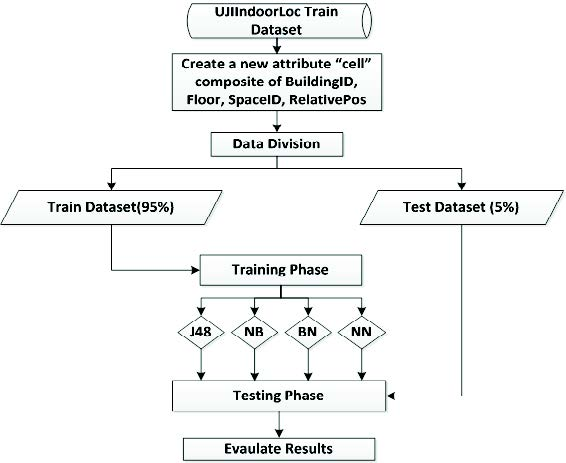
\includegraphics[scale=1]{figures/newattribute.jpg}
		\caption{The new attribute “cell” construction phase}
		\label{fig:newAttribute} %% NOTE: always label *after* caption!
	\end{center}
\end{figure}


\subsection{Algorithmes}
Dans la section suivante, les algorithmes de classification utilisés dans cette étude sont brièvement décrits.

\subsubsection{Decision Tree}
L'arbre de décisions et une méthode très connue en "machine learning". Il possède des noeuds de décisions (non-terminal), des branches, et des noeuds feuilles (terminal) qui représentent les caractéristiques, condition et les classes. A chaque noeud de décision on sait quelle branches suivre et lorsque l'algorithme atteint un noeud final, le label contenu dans ce même noeud est retourné comme étant la classe. 
L’ID3 de Quinlan et son successeur, C4.5, sont les plus populaires parmi les algorithmes d’arbre de décision [19].

(19) J. R. Quinlan, “ C4. 5: programs for machine learning”, Elsevier, 2014.

\subsubsection{Naïve Bayes}
Le classificateur Naïve Bayes [22] basé sur le théorème de Bayes est un algorithme d'apprentissage supervisé [23]. Il est robuste aux données bruyantes, facile à construire, affiche une grande précision et rapidité lorsqu'il est appliqué à de grandes bases de données et exécute des modèles de classification plus complexes. Par conséquent, il est largement utilisé dans les tâches de classification. Il calcule la probabilité de chaque attribut dans les données en supposant qu'elles sont également importantes et indépendantes les unes des autres. Cette hypothèse est appelée indépendance conditionnelle de classe [24, 25].
\\
\\
(22) G. H. John, and P. Langley, “Estimating Continuous Distributions in Bayesian Classifiers”, 11th Conference on Uncertainty in Artificial Intelligence, pp., 338-345, 1995.

(23) C. Anuradha, and S. Dhall, "Software Defect Prediction Using Supervised Learning Algorithm and Unsupervised Learning Algorithm", 2013.

(24) W. Yotsawat, and A. Srivihok, "Inbound tourists segmentation with combined algorithms using K-Means and Decision Tree”, 10th International Joint Conference on Computer Science and Software Engineering (JCSSE), pp.189-194, 2013.

(25) S. Ureerat, and P. Singsri, "The classifier model for prediction quail gender after birth based on external factors of quail egg", IEEE 11th International Joint Conference on Computer Science and Software Engineering (JCSSE), 2014.

\subsubsection{Bayesian Network}

L'algorithme de réseau bayésien est largement utilisé pour la classification et est basé sur le théorème de Bayes où la probabilité conditionnelle sur chaque nœud est calculée et forme un réseau bayésien. Il s'appelle également réseau de croyance ou réseau occasionnel. Réseau bayésien a deux parties nommées qualitatives et quantitatives, qui sont la structure topologique du réseau bayésien et le tableau de probabilité conditionnelle (CPT), respectivement [26].

Le réseau bayésien est un graphe acyclique dirigé où chaque nœud représente un attribut des données et un ensemble de distributions de probabilité. Ces distributions donnent les probabilités pour la valeur de chaque nœud étant donné que les parents de nœud.

(26) D. Yang, and L. Jin-lin, "Research on personal credit evaluation model based on bayesian network and association rules", 2007 International Conference on Wireless Communications, Networking and Mobile Computing, 2007.

\subsubsection{K-Nearest Neighbor}
Le classificateur K-Nearest Neighbor (K-NN) [27] est également connu sous le nom de classificateur basé sur la distance qui classe les instances en fonction de leur similarité. C'est l'un des algorithmes les plus populaires de l'apprentissage automatique. C'est un type d'apprentissage paresseux dans lequel la fonction n'est approchée que localement et tout calcul est retardé jusqu'à la classification. Le tuple inconnu dans K-NN est assigné à la classe la plus commune parmi ses K-plus proches voisins. Lorsque K = 1, le tuple inconnu se voit attribuer la classe du tuple d'apprentissage le plus proche dans l'espace des motifs [28].

(27) D. W. Aha, D. Kibler , and M. K. Albert, “ Instance-based learning algorithms”, Machine Learning, vol. 6, pp., 37-66, 1991.

(28) C. Shah, and A. G. Jivani, "Comparison of data mining classification algorithms for breast cancer prediction", 2013 Fourth International Conference on Computing, Communications and Networking Technologies (ICCCNT), pp.1-4, 2013.

\subsubsection{SMO}
L'algorithme d'optimisation séquentielle minimale (SMO - Sequential minimal optimization) [29] est représenté par John C. Platt pour la formation du classificateur de vecteurs de support à l'aide des noyaux polynomiaux ou RBF. C'est l'un des algorithmes les plus courants pour la classification des grandes marges par SVM. Il remplace globalement toutes les valeurs manquantes et transforme les attributs nominaux en attributs binaires. La SVM est une technique de classification basée sur la technologie des réseaux neuronaux utilisant la théorie de l'apprentissage statistique [30]. Il recherche un hyperplan optimal linéaire afin de maximiser la marge de séparation entre la classe positive et la classe négative. En pratique, la plupart des données ne sont pas linéairement séparables; ainsi, pour rendre la séparation possible, la transformation est effectuée à l'aide d'une fonction du noyau. L'entrée est transformée en un espace caractéristique de dimension supérieure à l'aide d'une cartographie non linéaire [30]. Une décision sur la fonction du Kernel est nécessaire pour implémenter SVM. Le Kernel définit la classe de fonction [31].

[29] J. Platt, “Fast Training of Support Vector Machines using Sequential Minimal Optimization”, Advances in Kernel Methods - Support Vector Learning, 1998.

[30] P. Niken, and H. Ohwada, "Applicability of machine-learning techniques in predicting customer defection", IEEE 2014 International Symposium on Technology Management and Emerging Technologies (ISTMET), 2014.

[31] S. M. Obaidullah, K. Roy, and N. Das, "Comparison of different classifiers for script identification from handwritten document", 2013 IEEE International Conference on Signal Processing, Computing and Control (ISPCC), pp.1-6, 2013.

\subsubsection{AdaBoost}
AdaBoost (Adaptive Boosting) [32] est un algorithme d'apprentissage d'ensemble. Généralement, il peut être utilisé avec des algorithmes de Machine learning faibles pour améliorer leurs performances. Il est simple à mettre en œuvre, rapide et moins susceptible d'avoir un overfitting. Il améliore les algorithmes de classification instables tels que J48, DecisionStump, etc. L'idée derrière cet algorithme est d'obtenir un classificateur très précis en combinant de nombreux classificateurs faibles. Il fonctionne en exécutant de manière répétée un algorithme d'apprentissage faible donné sur diverses distributions sur les données d'apprentissage, puis en combinant les classificateurs produits par l'apprenant faible en un classificateur composite unique [33]. Les classificateurs de l'ensemble sont ajoutés un par un, de sorte que chaque classificateur suivant est entrainé sur des données difficiles pour les membres précédents de l'ensemble. Les poids sont définis sur les instances du jeu de données, en suivant une règle selon laquelle les instances difficiles à classer prennent plus de poids. Cette règle conduit les classificateurs ultérieurs à se concentrer sur eux [34].

[32] Y. Freund, and R. E. Schapire, “Experiments with a new boosting algorithm”, 3th International Conference on Machine Learning, San Francisco, pp. 148-156, 1996.

[33] R. Shams, and R. E. Mercer, "Classifying Spam Emails Using Text and Readability Features", 2013 IEEE 13th International Conference on Data Mining (ICDM, pp. 657-666, 2013.

[34] S. O. Sharif, L. I. Kuncheva, and S. P. Mansoor, "Classifying encryption algorithms using pattern recognition techniques", 2010 IEEE International Conference on Information Theory and Information Security (ICITIS), , pp. 1168-1172, 2010.

\subsubsection{Bagging}
le Bagging [35] crée des sacs de données de la même taille que le jeu de données d'origine en appliquant une sélection aléatoire à différents sous-ensembles des données d'apprentissage avec de nombreux exemples qui apparaissent plusieurs fois. Ce processus est appelé réplication bootstrap des données d'entrainement. L'idée derrière cette technique est de construire différents classificateurs en utilisant ces sous-ensembles. Chaque sous-ensemble est utilisé pour entrainer un classificateur individuel. Cette approche d'ensemble utilise le nombre de classificateurs a priori [35].

[35] L. Breiman, “Bagging predictors”, Machine Learning. vol. 24, no. 2, pp.123-140, 1996.

\subsection{Conclusions}
Dans cet article les algorithme suivant ont été comparé : NN, SMO, J48, Naïve Bayes and BayesNet.

Lorsque tout le dataset est pris en compte, c'est l'algorithme J48 qui est le meilleur :

\begin{figure}[H]
	\begin{center}
		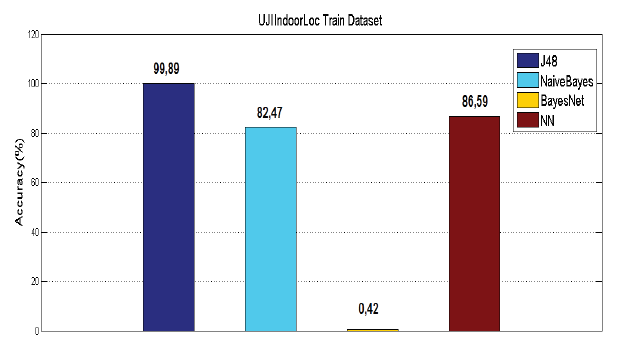
\includegraphics[scale=1]{figures/wholeDataset.png}
		\caption{Accuracy results of classification using whole dataset}
		\label{fig:wohledataset} %% NOTE: always label *after* caption!
	\end{center}
\end{figure}

Ensuite, en accordance à l'approche DESIP (Deductive Separation for Indoor Positioning), la classification est effectuée en 3 phases (building,floor and region). Le resultat des algorithme pour cette classification donne BayesNet comme étant le meilleur.

\begin{figure}[H]
	\begin{center}
		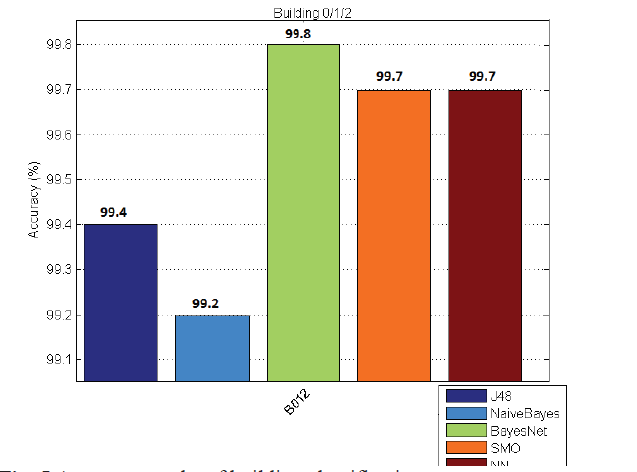
\includegraphics[scale=1]{figures/bluildingClassification.png}
		\caption{Accuracy results of building classification}
		\label{fig:builClass} %% NOTE: always label *after* caption!
	\end{center}
\end{figure}

Suite à cela la classification a été faite en fonction des étages (floors). Dans ce cas le meilleur algorithme est NN. 

\begin{figure}[H]
	\begin{center}
		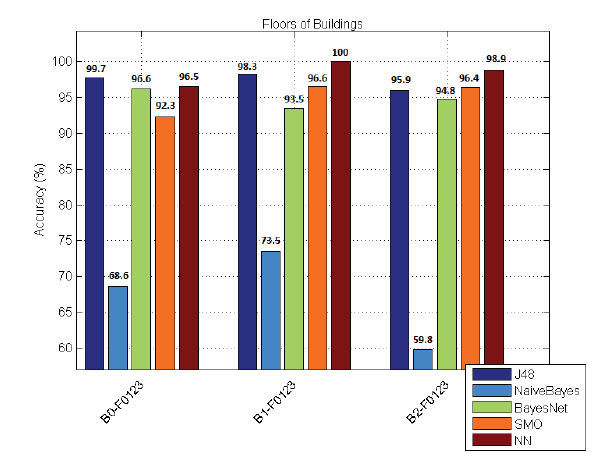
\includegraphics[scale=1]{figures/floorClassification.png}
		\caption{Accuracy results of floor classification}
		\label{fig:floorClass} %% NOTE: always label *after* caption!
	\end{center}
\end{figure}

Et pour la dernière étape, la classification a été faite en fonction de la région et là encore c'est l'algorithme NN qui est le meilleur.

\begin{figure}[H]
	\begin{center}
		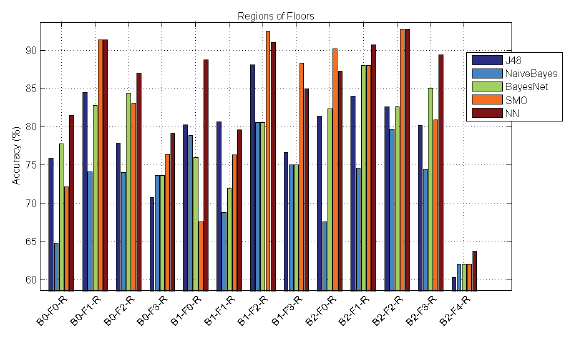
\includegraphics[scale=1]{figures/regionClassification.png}
		\caption{Accuracy results of region classification}
		\label{fig:regionClass} %% NOTE: always label *after* caption!
	\end{center}
\end{figure}

Si les deux tableaux ci-dessous sont analysés, l'algorithme NN est le meilleurs pour tous les dataset niveau temps d'execution. En ce qui concerne la précision, Bayes Net est meilleur pour la classification "building" par contre NN est meilleur dans tous les autres cas.

\begin{figure}[H]
	\begin{center}
		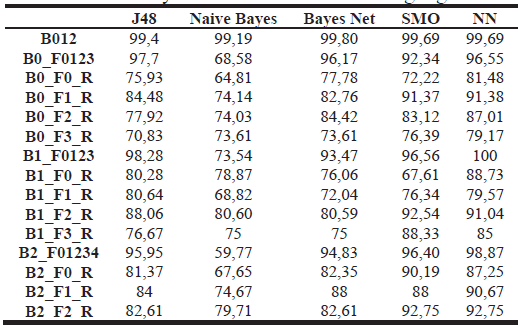
\includegraphics[scale=1]{figures/accuracy.png}
		\caption{Accuracy results of machine learning algorithms}
		\label{fig:accuracy} %% NOTE: always label *after* caption!
	\end{center}
\end{figure}

\begin{figure}[H]
	\begin{center}
		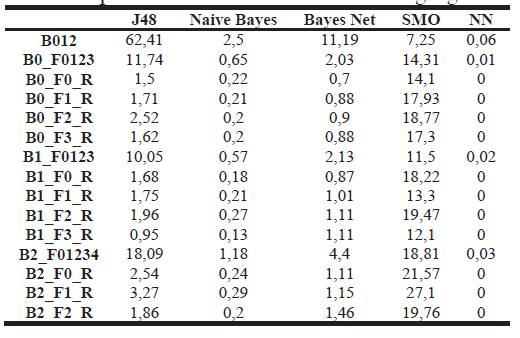
\includegraphics[scale=1]{figures/time.png}
		\caption{Elapsed time results of machine learning algorithms}
		\label{fig:time} %% NOTE: always label *after* caption!
	\end{center}
\end{figure}

De cette publication en découle que NN est supérieur à toutes les autres méthodes pour estimer la position. En outre, J48 offre des performances quasiment identiques lorsqu'il est utilisé avec des algorithmes itératifs, à savoir AdaBoost et Bagging.

\section{Résumé du document 02}
Cette publication traite de la diminution de erreur du mode ranging concernant la localisation UWB (ultra wide band). Plusieurs techniques existent pour diminuer l'erreur de positionnement en détectant ce qui est en ligne de vue (LOS) ou non (NLOS). Ici, il est exploité une autre technique qui va directement diminuer cet erreur que ça soit en LOS ou NLOS. Ils appliquent deux classes de régresseurs non paramétriques pour avoir une estimation de l'erreur de mesure. Afin de valider leurs résultats ils ont fait un vaste campagne de mesures intérieures. Cette technique montre une amélioration de performances significatives dans divers scénarios par rapport aux approches conventionnelles. 

Ils se sont appuyé sur des outils de Machine Learning, et proposent deux techniques de régression non paramétriques pour estimer l’erreur de mesure, en se basant uniquement sur la forme d’onde reçue et la distance estimée.


\begin{enumerate}
	\item La première technique utilise une régression de machine à vecteurs de support (SVM - support vector machine) pour trouver un hyperplan qui se rapproche de l'erreur de mesure en fonction des données d'apprentissage. 
	\item La seconde technique utilise un processus gaussien (GP) pour déterminer la distribution a posteriori de l'erreur de mesure, en fonction des données d'apprentissage. 
\end{enumerate}

L'erreur de mesure estimée, associée à une mesure de certitude, peut être transmise à un algorithme de localisation. Leurs techniques de régression présentent l'avantage supplémentaire de pouvoir être appliquées même lorsque les données d'apprentissage ne sont pas étiquetées avec des informations LOS ou NLOS.

\subsection{Ranging Errors}
Lors de mesure il existe beaucoup de paramètres qui peuvent créer une erreur. Avec un seul model il est difficile de capturer tout les types de perturbations. Dans cette publication, ils se basent sur 1024 mesures (512 LOS et 512 NLOS).

\begin{figure}[H]
	\begin{center}
		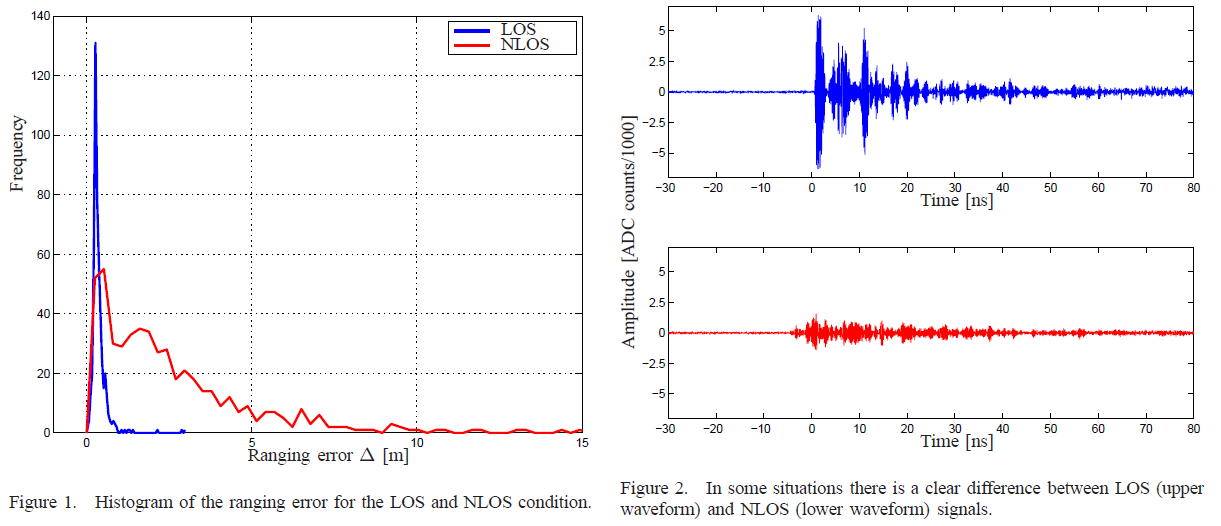
\includegraphics[scale=1]{figures/LosNlos.png}
		\caption{Ranging error - LOS and NLOS}
		\label{fig:LosNlos} %% NOTE: always label *after* caption!
	\end{center}
\end{figure}

Suite, aux différentes mesures et différentes observations dans leur article, ils décident de ne pas labéliser les signaux en LOS et NLOS.

\subsection{Algrorithme}
\subsubsection{Regression with Support Vector Machines}
\subsubsection{Regression with Gaussian Processes}

\subsection{Conclusion}
Les approches classiques pour faire face au défi de la localisation dans des environnements encombrés impliquent généralement d'abord la détection de la condition NLOS, puis la prise de mesures appropriées pour prendre en compte la condition NLOS. Toutefois, la grande variété de matériaux et d’environnements d’exploitation variés peuvent impacter les performances de la mesure de ranging, ce qui indique que la distinction entre LOS et NLOS n’est pas toujours significative. Sur la base de cette observation, ils ont adopté pour une approche différente dans cet article. Leur approche utilise des techniques de Machine Learning non paramétriques (SVM et GP) pour estimer l’erreur de "ranging" directement à partir de la forme d’onde reçue, sans aucune connaissance a priori ou a posteriori de la condition NLOS. 

Sur la base d'une vaste campagne de mesures en intérieur avec des radios UWB conformes à la FCC, ils ont évalué les performances de localisation en termes de probabilité de panne pour différentes stratégies de localisation. Leurs résultats ont révélé que: 

\begin{enumerate}
	\item La minimisation de l1-norme est plus robuste pour faire face aux valeurs aberrantes (outliers) que la minimisation de l2-norme, pour une localisation sans atténuation.
	\item les contraintes peuvent générer des gains significatifs, en particulier lorsque les exigences de localisation ne sont pas trop strictes.
	\item les techniques de régression SVM ou GP offrent des gains de performance supplémentaires pour tous les scénarios considérés.
	\item Les techniques de régression SVM ou GP, combinées à la connaissance des contraintes relatives à l'erreur de "ranging", offrent les meilleures performances pour les scénarios considérés.
\end{enumerate}

\section{Résumé du document 03}
\subsection{Pro/con}
%\chapter{Rapport intérmédiaire : 15.10.2018 au 26.10.2018}

\section{Objectifs et tâches à réaliser}

%\begin{enumerate}
%	\item fgfd
%	\item gdgfd
%\end{enumerate}


%\begin{figure}[H]
%	\begin{center}
%		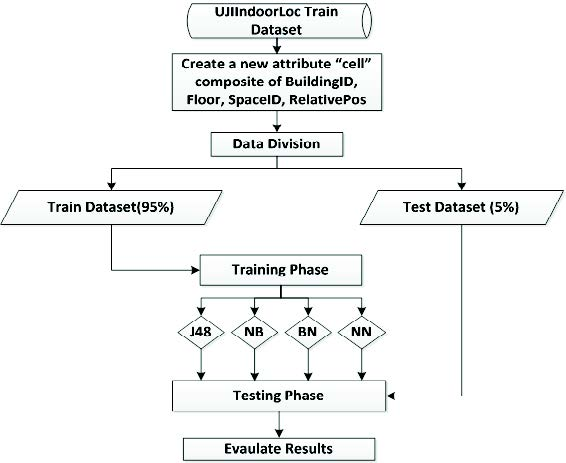
\includegraphics[scale=1]{figures/newattribute.jpg}
%		\caption{The new attribute “cell” construction phase}
%		\label{fig:newAttribute} %% NOTE: always label *after* caption!
%	\end{center}
%\end{figure}

%\todo{Compléter cette partie qui semble importante}

\include{chapter/000_introduction}
\chapter{État de l'art}
Ce chapitre passe en revue les solutions existantes qui parlent d'application des méthodes d'apprentissage pour l'amélioration de la précision de la localisation intérieure. L'exploration de ces sujets va permettre de choisir la solution la plus adaptée pour remplir les objectifs de ce travail.

Pour ce faire, quatre ouvrages ont été étudiés. Les trois premiers traitent du positionnement intérieur aidé avec des algorithmes d'apprentissage (Machine Learning). Le quatrième a été sélectionné, car il traite de la gestion de "outliers", c'est à dire comment détecter des points aberrants et qui pourraient fausser les mesures. 

Grâce à l'étude des structures existantes, une première classification selon le type d'apprentissage et selon les algorithmes de classification utilisés peut être établie. En plus, un aperçu de la façon de détecter les "outliers" est soulevé.

\section{Classification des algorithmes d'apprentissage}
Il existe plusieurs catégories d'estimateur et dans ces catégories, il y a plusieurs algorithmes à choix. La Figure \ref{fig:scikiLearn} permet de sélectionner différents algorithmes en fonction de ce qu'il est nécessaire d'obtenir. On remarque sur cette figure qu'il y a quatre groupes distincts : classification, regression, clustering et dimensionality reduction. En partant depuis le point "start" et en répondant aux différentes questions, cela va proposer un algorithme qui permet de répondre à nos besoins.

\begin{figure}[htp]
 \begin{center}
  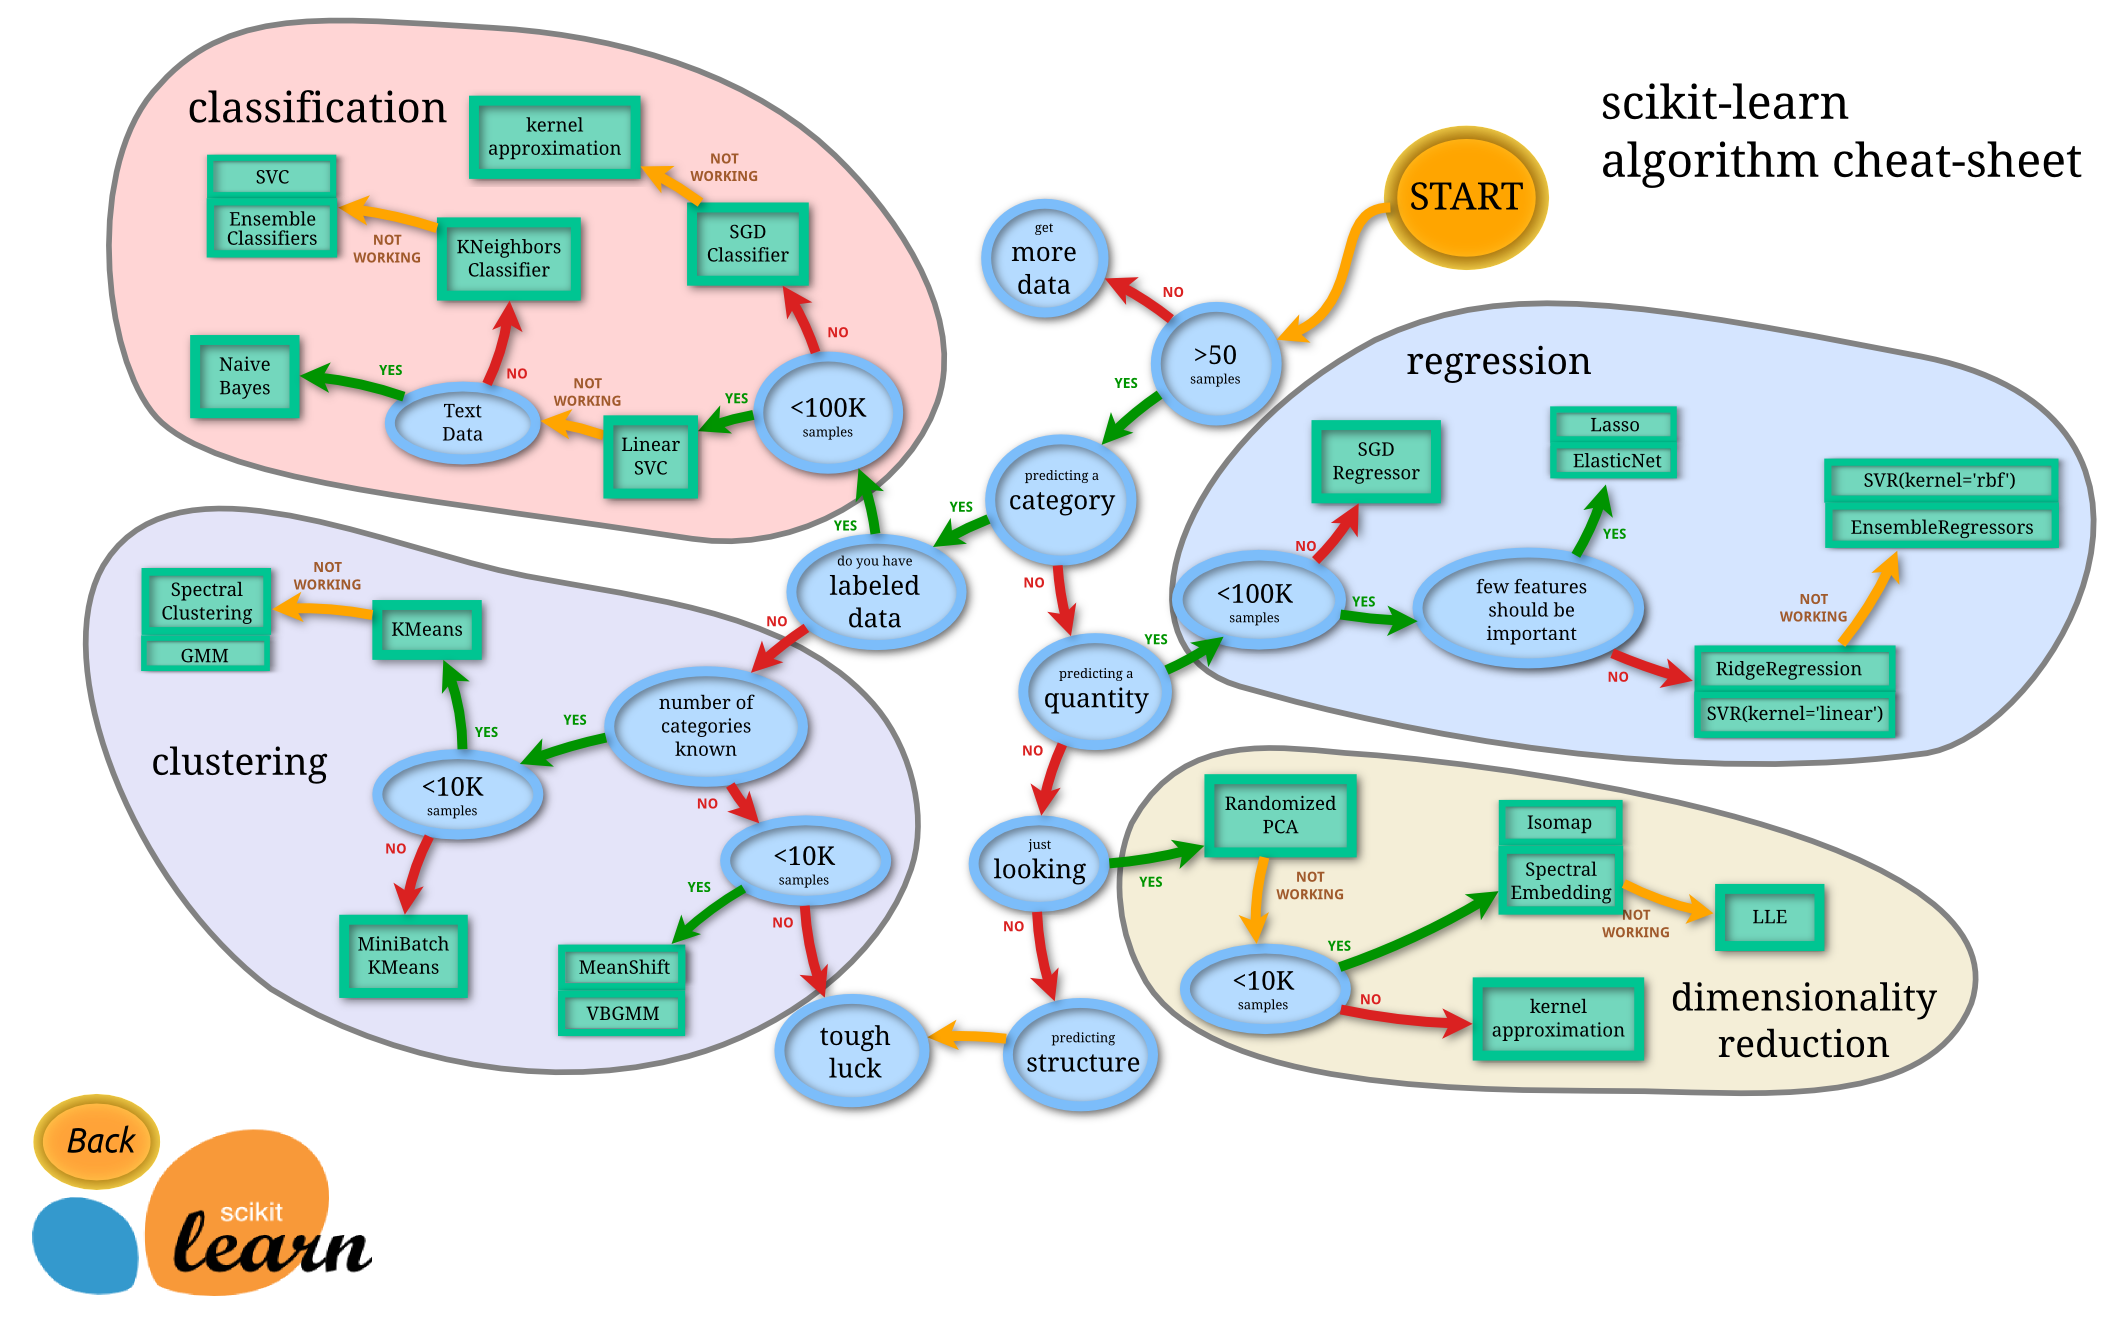
\includegraphics[scale=0.12]{figures/scikiLearn.png}
  \caption{Comment choisir un algorithme ML \cite{scikit}}
  \label{fig:scikiLearn} %% NOTE: always label *after* caption!
 \end{center}
\end{figure}

Dans le cas de ce travail, il y a deux possibilités, soit d'utiliser une classification soit d'utiliser une régression. Dans la Figure \ref{fig:ClassReg}, on peut visualiser la différence entre les deux types d'estimateurs. Dans le cas de la classification, on va apprendre à notre algorithme différentes positions et l'algorithme sera ensuite capable de fournir en sortie une de ses positions. Donc, il sort une région plutôt qu'une coordonnée. Si l'entrainement de l'algorithme a été fait avec un maillage fin alors le résultat sera fin. Lorsqu'un point est détecté, il sera classifié selon la position la plus proche comme on le voit sur la Figure \ref{fig:ClassReg} avec le carré vert et le carré rouge. Dans une régression, la problématique est un peu différente. L'algorithme sera également entrainé avec différentes positions, mais ensuite, par régression l'algorithme va tenter d'estimer la position du nouveau point en calculant sa coordonnée alors que pour une classification il s’agit de positionner ce nouveau point dans une classe. 

\begin{figure}[htp]
 \begin{center}
  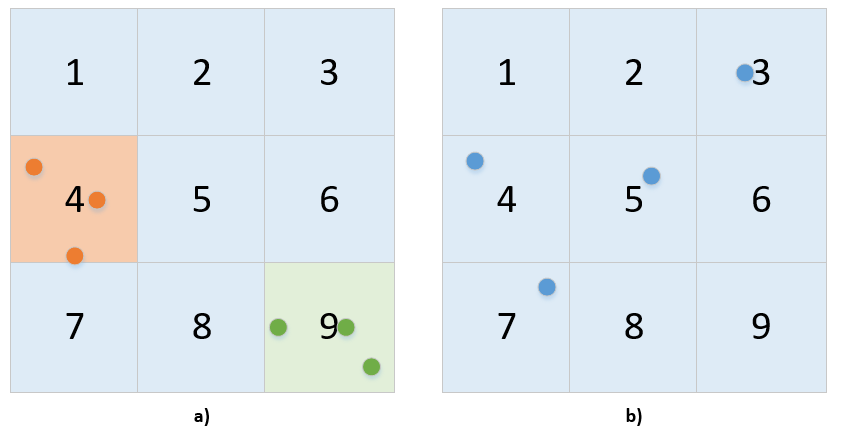
\includegraphics[scale=0.5]{figures/ClassReg.png}
  \caption{a) exemple de classification  b) exemple de régression}
  \label{fig:ClassReg} %% NOTE: always label *after* caption!
 \end{center}
\end{figure}

\section{Algorithme de classification}
Dans cette section, quelques algorithmes de classification utilisés dans ces études \cite{ML_indoor} \cite{CP_RSS} sont brièvement décrits et analysés.

\subsection{Decision Tree}
L'arbre de décisions et une méthode très connue en "machine learning". Il possède des noeuds de décisions (non-terminal), des branches, et des noeuds feuilles (terminal) qui représentent les caractéristiques, condition et les classes. À chaque noeud de décision on sait quelles branches suivre et lorsque l'algorithme atteint un noeud final, le label contenu dans ce même noeud est retourné comme étant la classe. 
L’ID3 de Quinlan et son successeur, C4.5, sont les plus populaires parmi les algorithmes d’arbre de décision \cite{C4_5}.

\subsection{Naïve Bayes}
Le classificateur Naïve Bayes \cite{Bayesian} basé sur le théorème de Bayes est un algorithme d'apprentissage supervisé \cite{DefectPred}. Il est robuste aux données bruyantes, faciles à construire, affiche une grande précision et rapidité lorsqu'il est appliqué à de grandes bases de données et exécute des modèles de classification plus complexes. Par conséquent, il est largement utilisé dans les tâches de classification. Il calcule la probabilité de chaque attribut dans les données en supposant qu'elles sont également importantes et indépendantes les unes des autres. Cette hypothèse est appelée indépendance conditionnelle de classe \cite{KMean_DT} \cite{QUAIL}.

\subsection{Bayesian Network}
L'algorithme de réseau bayésien est largement utilisé pour la classification et est basé sur le théorème de Bayes où la probabilité conditionnelle sur chaque nœud est calculée et forme un réseau bayésien. Il s'appelle également réseau de croyance ou réseau occasionnel. Le réseau bayésien à deux parties nommées qualitatives et quantitatives, qui sont la structure topologique du réseau bayésien et respectivement le tableau de probabilité conditionnelle (CPT) \cite{Bayesian01}.

Le réseau bayésien est un graphe acyclique dirigé où chaque nœud représente un attribut des données et un ensemble de distributions de probabilité. Ces distributions donnent les probabilités pour la valeur de chaque nœud.

\subsection{K-Nearest Neighbor}
Le classificateur K-Nearest Neighbor (K-NN) \cite{ML00} est également connu sous le nom de classificateur basé sur la distance qui classe les instances en fonction de leur similarité. C'est l'un des algorithmes les plus populaires de l'apprentissage automatique. C'est un type d'apprentissage paresseux dans lequel la fonction n'est approchée que localement et tout calcul est retardé jusqu'à la classification. Le point inconnu dans K-NN est assigné à la classe la plus commune parmi ses K-plus proches voisins. Lorsque K = 1, le point inconnu se voit attribuer la classe du point d'apprentissage le plus proche dans l'espace des motifs \cite{ML01}.

\subsection{SMO / SVM}
L'algorithme d'optimisation séquentielle minimale (SMO - Sequential minimal optimization) \cite{ML29} est représenté par John C. Platt pour la formation du classificateur de vecteurs de support à l'aide des noyaux polynomiaux ou RBF. C'est l'un des algorithmes les plus courants pour la classification des grandes marges par SVM. Il remplace globalement toutes les valeurs manquantes et transforme les attributs nominaux en attributs binaires. SVM est une technique de classification basée sur la technologie des réseaux de neuronnes utilisant la théorie de l'apprentissage statistique \cite{ML30}. Il recherche un hyperplan optimal linéaire afin de maximiser la marge de séparation entre la classe positive et la classe négative. En pratique, la plupart des données ne sont pas linéairement séparables; ainsi, pour rendre la séparation possible, la transformation est effectuée à l'aide d'une fonction du noyau. L'entrée est transformée en un espace caractéristique de dimensions supérieures à l'aide d'une cartographie non linéaire. Une décision sur la fonction du Kernel est nécessaire pour implémenter SVM. Le Kernel définit la classe de fonction \cite{ML31}.

\subsection{AdaBoost}
AdaBoost (Adaptive Boosting) \cite{ML32} est un algorithme d'apprentissage d'ensemble. Généralement, il peut être utilisé avec des algorithmes de Machine learning faibles pour améliorer leurs performances. Il est simple à mettre en œuvre, rapide et moins susceptible d'avoir un overfitting. Il améliore les algorithmes de classification instables tels que J48, DecisionStump, etc. L'idée derrière cet algorithme est d'obtenir un classificateur très précis en combinant de nombreux classificateurs faibles. Il fonctionne en exécutant de manière répétée un algorithme d'apprentissage faible donné sur diverses distributions sur les données d'apprentissage, puis en combinant les classificateurs produits par l'apprenant faible en un classificateur composite unique \cite{ML33}. Les classificateurs de l'ensemble sont ajoutés un par un, de sorte que chaque classificateur suivant est entrainé sur des données difficiles pour les membres précédents de l'ensemble. Les poids sont définis sur les instances du jeu de données, en suivant une règle selon laquelle les instances difficiles à classer prennent plus de poids. Cette règle conduit les classificateurs ultérieurs à se concentrer sur eux \cite{ML34}.

\subsection{Bagging}
Le Bagging \cite{ML35} crée des sacs de données de la même taille que le jeu de données d'origine en appliquant une sélection aléatoire à différents sous-ensembles des données d'apprentissage avec de nombreux exemples qui apparaissent plusieurs fois. Ce processus est appelé réplication bootstrap des données d'entrainement. L'idée derrière cette technique est de construire différents classificateurs en utilisant ces sous-ensembles. Chaque sous-ensemble est utilisé pour entrainer un classificateur individuel. Cette approche d'ensemble utilise le nombre de classificateurs a priori \cite{ML35}.

\section{Algorithme de régression}
Dans cette section, quelques algorithmes de régression utilisés dans cette étude \cite{ML_UWB} sont brièvement décrits et analysés.

\subsection{Support Vector Machine pour la régression (SVR)}
Support Vector Machine (SVM) est une méthode d'apprentissage supervisée utilisée pour la classification. Cette méthode peut être étendue pour résoudre des problèmes de régression et cette méthode s'appelle Support Vetor Regression (SVR).

Systeme Vector Regression (SVR) est considéré comme une technique non paramétrique, car il dépend du Kernel. 

Il existe trois implémentations différentes de Support Vector Regression: SVR, NuSVR et LinearSVR. LinearSVR fournit une implémentation plus rapide que SVR, mais ne considère que les noyaux linéaires, tandis que NuSVR implémente une formulation légèrement différente de SVR et de LinearSVR.\cite{scikit}

\subsection{Gaussian Process (GP)}
Gaussian processes a récemment gagné en intérêt du côté des algorithmes d'apprentissage. Cela, car il forme un bon framework pour résoudre des problèmes de régression \cite{ML51}.

C'est une méthode d'apprentissage supervisée pour résoudre des problèmes de régression comme dit ci-dessus, mais également des problèmes de probabilités. 

Les avantages du processus gaussien sont:

\begin{enumerate}
 \item La prédiction interpole les observations (au moins pour les noyaux normaux).
 \item La prédiction est probabiliste (gaussienne) afin que l’on puisse calculer des intervalles de confiance empiriques et décider en fonction de ceux-ci s’il convient de réajuster (adaptation en ligne, adaptation adaptative) la prévision dans une région d’intérêt.
 \item Polyvalent: différents noyaux peuvent être spécifiés. Les noyaux communs sont fournis, mais il est également possible de spécifier des noyaux personnalisés.
\end{enumerate}

Les inconvénients des processus gaussiens sont:

\begin{enumerate}
 \item Ils ne sont pas clairsemés, c’est-à-dire qu’ils utilisent l’ensemble des informations sur les échantillons / caractéristiques pour effectuer la prédiction.
 \item Ils perdent leur efficacité dans les espaces de grandes dimensions, notamment lorsque le nombre de caractéristiques dépasse quelques dizaines.
\end{enumerate} 

\cite{scikit}. 

\section{ Détection d'outliers \cite{ML_indoor}}
Cette section donne un aperçu de la manière de traiter les "outliers - valeurs aberrantes", c'est-à-dire les points qui ne sont pas cohérents lors d'une mesure. Selon Barnet et Lewis \cite{Outliers}, un "outliers" est défini comme étant une observation qui semble incompatible avec le reste d'un ensemble de données.
Garder un "outliers" dans un jeu de données peut amener à de mauvais résultats, il est donc important de les détecter correctement. Il existe différentes méthodes pour déterminer ces "outliers" :

\begin{enumerate}
 \item Grubbs' test : détecte un "outliers" en supposant une distribution normale.
 \item Tietjen-Moore test : C'est une généralisation de Grubbs' test pour détecter de multiple outliers. Il a cependant un inconvénient, il est nécessaire de connaitre le nombre exact d'ouliers.
 \item Generalized Extreme Studentized Deviate (ESD): c'est également une généralisation du test Grubbs', mais il n'est pas nécessaire de connaitre à l'avance le nombre d'ouliers. Ce test nécessite uniquement une limite supérieure pour le nombre suspect d'outliers.\cite{ESD}
\end{enumerate}

\section{Étude des travaux existants}
Les trois documents ne peuvent pas être comparés à proprement dit, car ils traitent de différentes manières. Un parle d'algorithme de classification et compare différents algorithmes existants. Un autre document traite de régression et compare également différents algorithmes. Le dernier document parle de la prédiction conforme (CP - conformal prediction) qui va permettre d'améliorer encore les résultats avec un algorithme choisi.  

C'est pourquoi les documents sont résumés en mettant les points importants en évidence séparément. Ils seront décrits plutôt que comparés. 

\subsection{Analyse comparative de différents algorithmes pour le positionnement intérieur \cite{ML_algo}}
Cette publication parle d'une analyse comparative entre différents algorithmes de "machine learning" pour du positionnement intérieur. L'étude est basée sur un positionnement "fingerprint" ce qui permet de cartographier un endroit à l'aide de la force du signal réceptionné (RSS - Received Signal Strength).
Dans cet article, les algorithmes de "machine learning" sélectionnés sont comparés en termes de précision de positionnement et de temps de calcul. 

Au cours des expériences, la base de données UJIIndoorLoc est utilisée. La classification est effectuée en premier lieu en utilisant le jeu de données d'origine en considérant les valeurs RSS des 520 points d'accès sans fil (WAP - wireless access points) et les nouveaux attributs définis en tant que «cellule» qui composent les attributs : BuildingID, Floor, SpaceID et RelativePos. Ensuite, une nouvelle méthode est proposée: «Séparation déductive pour le positionnement intérieur (DESIP - Deductive Separation for Indoor Positioning)». Dans cette méthode, tout d'abord, seules les informations de bâtiment et les valeurs RSS mesurées à partir de 520 WAP sont utilisées pour la tâche de classification.

Durant les expériences, des algorithmes tels que le plus proche voisin (NN - nearest neighbor), le SMO, l'arbre de décision (J48), Naïve Bayes et Bayes Net sont utilisés. L’algorithme le plus approprié pour la solution du problème de positionnement intérieur est déterminé en comparant la précision et le temps de calcul de chaque approche.

La base de données entière est séparée de telle sorte que 19'937 enregistrements soient réservés à l'apprentissage et 1'111 enregistrements soient réservés aux tests. Il y a 529 caractéristiques qui sont: les coordonnées où sont prises les empreintes digitales WiFi, telles que bâtiment, étage, espace (bureau, laboratoire, etc.), position relative (dans une pièce ou dans un couloir), etc. Le jeu de données d'apprentissage UJIIndoorLoc comprenant les valeurs RSSI de 520 WAP et une autre «cellule» qui comprend les attributs floor, buildingID, spaceID et relative position de l'ensemble de données d'origine est utilisé pour la tâche de classification. Les étapes des expériences utilisant ce jeu de données sont illustrées à la Figure \ref{fig:newAttribute}. Dans un premier temps, le jeu de données (dataset) est séparé en deux groupes. Un groupe est utilisé pour l'apprentissage (train dataset) et l'autre partie est utilisée pour valider le résultat des différents algorithmes (test dataset). Le jeu d'entrainement est utilisé pour quatre différents algorithmes.

\begin{figure}[htp]
 \begin{center}
  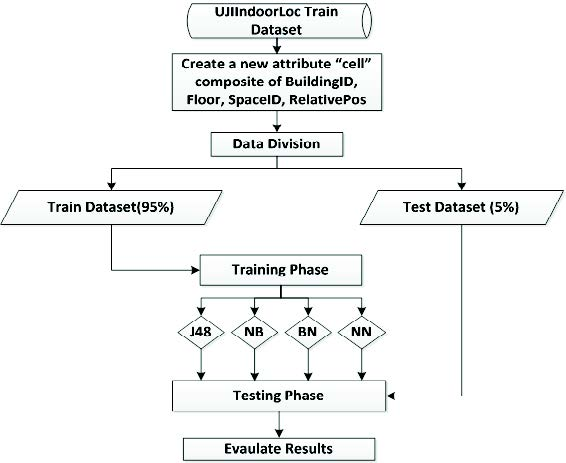
\includegraphics[scale=0.7]{figures/newattribute.jpg}
  \caption{Phase de construction et d'apprentissage \cite{ML_algo}}
  \label{fig:newAttribute} %% NOTE: always label *after* caption!
 \end{center}
\end{figure}

Dans cet article, les algorithmes suivants ont été comparés dans différentes situations: NN, SMO, J48, Naïve Bayes et BayesNet. La classification est effectuée en trois phases (building,floor and region). La première étape est la classification par bâtiment (Figure \ref{fig:builClass}). Le résultat des algorithmes pour cette classification donne BayesNet comme étant le meilleur, car il possède la meilleure précision.

\begin{figure}[htp]
 \begin{center}
  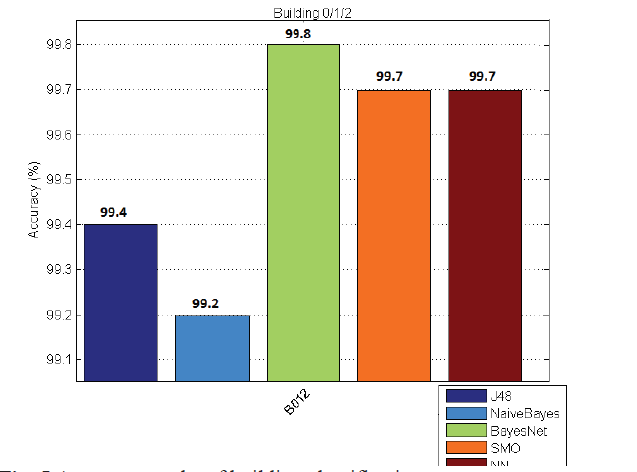
\includegraphics[scale=0.6]{figures/bluildingClassification.png}
  \caption{Résultats des précisons pour la classification par bâtiments \cite{ML_algo}}
  \label{fig:builClass} %% NOTE: always label *after* caption!
 \end{center}
\end{figure}

Suite à cela, la classification a été faite en fonction des étages (floors) (Figure \ref{fig:floorClass}). Dans ce cas, le meilleur algorithme est NN. 

\begin{figure}[htp]
 \begin{center}
  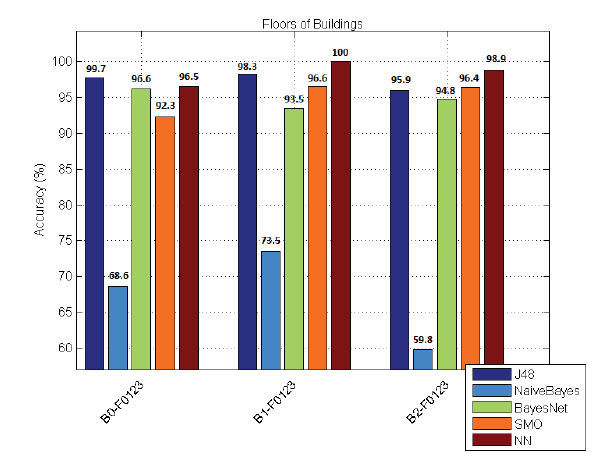
\includegraphics[scale=0.6]{figures/floorClassification.png}
  \caption{Résultats de la précision pour la classification par étage.\cite{ML_algo}}
  \label{fig:floorClass} %% NOTE: always label *after* caption!
 \end{center}
\end{figure}

Et pour la dernière étape (Figure \ref{fig:regionClass}), la classification a été faite en fonction de la région et là encore, c'est l'algorithme NN qui est le meilleur.

\begin{figure}[htp]
 \begin{center}
  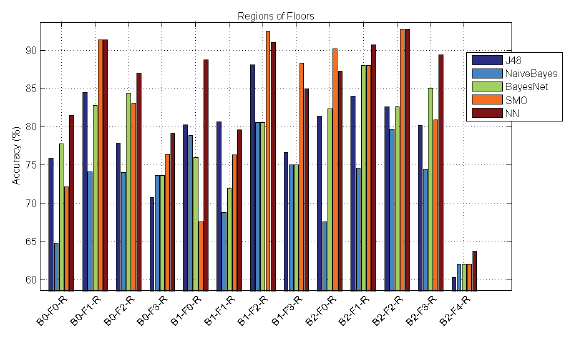
\includegraphics[scale=0.6]{figures/regionClassification.png}
  \caption{Résultats de la précision pour la classification par région. \cite{ML_algo}}
  \label{fig:regionClass} %% NOTE: always label *after* caption!
 \end{center}
\end{figure}

Les deux tableaux (Figure \ref{fig:accuracy} et Figure \ref{fig:time}) permettent d'avoir une vue d'ensemble de tous les algorithmes appliqués et leur performance en termes de précision et de rapidité. L'algorithme NN est le meilleur pour tous les jeux de données au niveau du temps d'exécution. En ce qui concerne la précision, Bayes Net est meilleur pour la classification "building" par contre NN est meilleur dans tous les autres cas.

\begin{figure}[htp]
 \begin{center}
  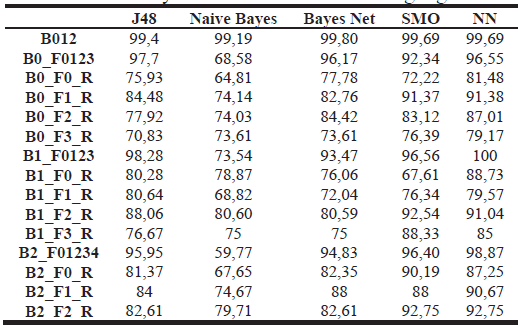
\includegraphics[scale=1]{figures/accuracy.png}
  \caption{Résultat de la précision des algorithmes d'apprentissage.\cite{ML_algo}}
  \label{fig:accuracy} %% NOTE: always label *after* caption!
 \end{center}
\end{figure}

\begin{figure}[htp]
 \begin{center}
  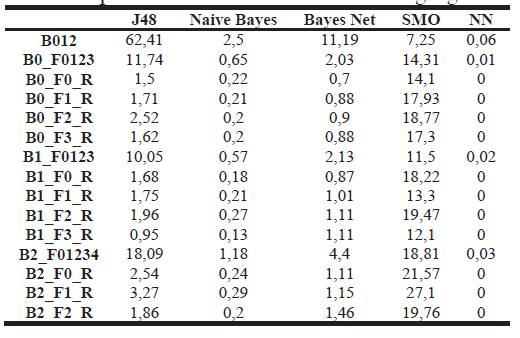
\includegraphics[scale=1]{figures/time.png}
  \caption{Résultats du temps de traitement des algorithmes d'apprentissage\cite{ML_algo}}
  \label{fig:time} %% NOTE: always label *after* caption!
 \end{center}
\end{figure}

Les résultats expérimentaux révèlent que l’algorithme k-Nearest Neighbor (k-NN) est le plus approprié lors du positionnement. En outre, J48 offre des performances quasiment identiques lorsqu'il est utilisé avec des algorithmes itératifs, à savoir AdaBoost et Bagging. Il est à noter que toutes ces méthodes mettent en évidence des classifications. C'est-à-dire que le résultat placera un nouveau point sur l'un des points entrainé et ne donne pas une nouvelle coordonnée comme cela serait le cas d'un résultat par régression. 

\subsection{Machine learning pour diminuer l'erreur de positionnement UWB \cite{ML_UWB}}
Les approches classiques pour faire face au défi de localisation dans des environnements encombrés impliquent généralement d'abord la détection de la condition NLOS (NLOS = pas en ligne de vue), puis la prise de mesures appropriées pour prendre en compte la condition NLOS. Toutefois, la grande variété de matériaux et d’environnements d’exploitation variés peuvent impacter les performances de la mesure de ranging, ce qui indique que la distinction entre LOS et NLOS n’est pas toujours significative. Sur la base de cette observation, ils ont opté pour une approche différente dans cet article. Leur approche utilise des techniques de Machine Learning non paramétriques (SVM et GP) pour estimer l’erreur de "ranging" directement à partir de la forme d’onde reçue, sans aucune connaissance a priori ou a posteriori de la condition NLOS. 

Cette publication traite de la diminution de l'erreur du mode ranging concernant la localisation UWB (Ultra Wide Band). Plusieurs techniques existent pour diminuer l'erreur de positionnement en détectant ce qui est en ligne de vue (LOS) ou non (NLOS). Ici, une autre technique est exploitée et va directement diminuer cette erreur que ça soit en LOS ou en NLOS. Ils appliquent deux classes de régresseurs non paramétriques pour avoir une estimation de l'erreur de mesure. Afin de valider leurs résultats, ils ont fait une vaste campagne de mesures intérieures. Cette technique montre une amélioration de performances significatives dans divers scénarios par rapport aux approches conventionnelles. 

La régression non paramétrique est une forme d'analyse de la régression dans laquelle le prédicteur, ou fonction d'estimation ne prend pas de forme prédéterminée, mais est construite selon les informations provenant des données. La régression non paramétrique exige des tailles d'échantillons plus importantes que celles de la régression basée sur des modèles paramétriques parce que les données doivent fournir la structure du modèle ainsi que les estimations du modèle. \cite{WIKI1}

Ils se sont appuyés sur des outils d'apprentissage (Machine Learning), et proposent deux techniques de régression pour estimer l’erreur de mesure, en se basant uniquement sur la forme d’onde reçue et la distance estimée.

\begin{enumerate}
 \item La première technique utilise une régression SVM (support vector machine) pour trouver un hyperplan qui se rapproche de l'erreur de mesure en fonction des données d'apprentissage. 
 \item La seconde technique utilise un processus gaussien (GP) pour déterminer la distribution a posteriori de l'erreur de mesure, en fonction des données d'apprentissage. 
\end{enumerate}

L'erreur de mesure estimée, associée à une mesure de certitude, peut être transmise à un algorithme de localisation. Leurs techniques de régression présentent l'avantage supplémentaire de pouvoir être appliquées même lorsque les données d'apprentissage ne sont pas étiquetées avec des informations LOS ou NLOS.

Lors des mesures, il existe beaucoup de paramètres qui peuvent créer une erreur. Avec un seul modèle, il est difficile de capturer tous les types de perturbations. Dans cette publication, ils se basent sur 1024 mesures (512 LOS et 512 NLOS) Figure \ref{fig:LosNlos}.

\begin{figure}[htp]
 \begin{center}
  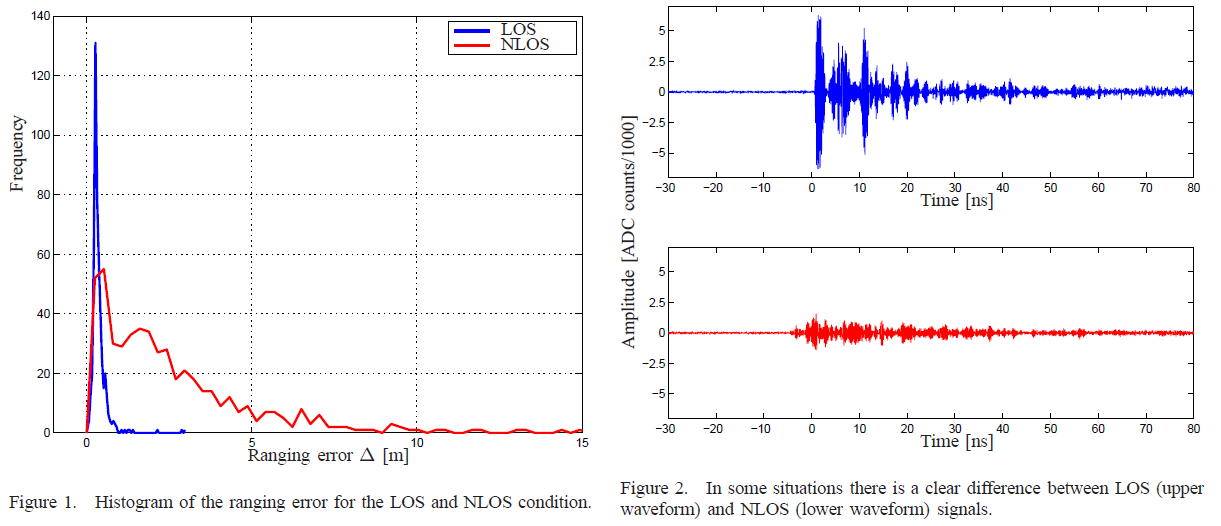
\includegraphics[scale=0.6]{figures/LosNlos.png}
  \caption{Ranging error - LOS and NLOS \cite{ML_UWB}}
  \label{fig:LosNlos} %% NOTE: always label *after* caption!
 \end{center}
\end{figure}

Sur la base d'une vaste campagne de mesures en intérieur avec des radios UWB conformes à la FCC (Federal Communications Commission), ils ont évalué les performances de localisation en termes de probabilité de panne pour différentes stratégies de localisation. Leurs résultats ont révélé que: 

\begin{enumerate}
 \item La minimisation de l1-norme est plus robuste pour faire face aux valeurs aberrantes (outliers) que la minimisation de l2-norme, pour une localisation sans atténuation.
 \item les contraintes peuvent générer des gains significatifs, en particulier lorsque les exigences de localisation ne sont pas trop strictes.
 \item les techniques de régression SVM ou GP offrent des gains de performance supplémentaires pour tous les scénarios considérés.
 \item Les techniques de régression SVM ou GP, combinées à la connaissance des contraintes relatives à l'erreur de "ranging", offrent les meilleures performances pour les scénarios considérés.
\end{enumerate}

\subsection{Amélioration du positionnement en utilisant "conformal prediction" \cite{CP_RSS}}
Pareil que dans les deux précédentes publications, le but est d'améliorer la précision du positionnement intérieur où il n'est pas possible d'utiliser un GPS. Cela toujours en tenant compte des problématiques d'un environnement dynamique avec des personnes qui bougent et de l'environnement complexe avec des murs, etc.. Dans cet article, ils ont validé leur solution dans trois immeubles. Cet article est basé sur un positionnement WIFI fingerprinting et se base sur la force du signal reçu (RSSI).

Pour effectuer les mesures il y a deux phases voir Figure \ref{fig:Fingerprinting}. 

\begin{figure}[htp]
 \begin{center}
  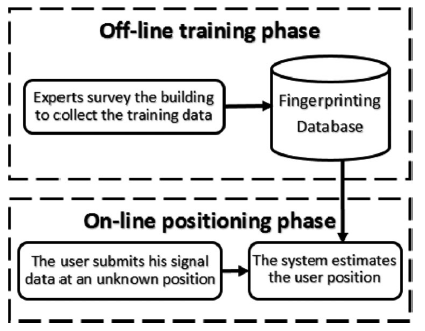
\includegraphics[scale=1]{figures/Fingerprinting.png}
  \caption{Les deux phases du fingerprinting}
  \label{fig:Fingerprinting} %% NOTE: always label *after* caption!
 \end{center}
\end{figure}

La première phase (Off-line training) consiste à décider combien de mesures nous voulons faire (tous les mètres? centimètres?), comment sont prises les mesures (plusieurs mesures sont faites à chaque position) et comment labéliser le signal (souvent labélisé avec la coordonnée réelle). Cette phase est très importante et il est nécessaire de bien réfléchir comment procéder (utiliser un robot par exemple). C'est ce qu'on appelle la phase d'entrainement.

Concernant la seconde phase (on-line positioning), c'est de définir le positionnement. Durant cette phase la partie délicate est de définir quel algorithme utiliser. C'est durant cette phase que les algorithmes seront testés. 

Il existe une compétition comparative pour les positionnements intérieurs (Microsoft IPSN 2014) Figure \ref{fig:Competition}.

Une localisation précise à l'intérieur peut potentiellement transformer la façon dont les gens naviguent à l'intérieur, de la même manière que le GPS a transformé la façon dont les gens naviguent à l'extérieur. Au cours des 15 dernières années, le monde universitaire et l’industrie ont proposé et expérimenté plusieurs technologies de localisation en intérieur, mais nous n’avons pas encore assisté à des déploiements à grande échelle. Ce concours vise à rassembler des technologies de localisation intérieure en temps réel ou quasi réel et à comparer leurs performances dans le même espace. \cite{MICRO}

\begin{figure}[htp]
 \begin{center}
  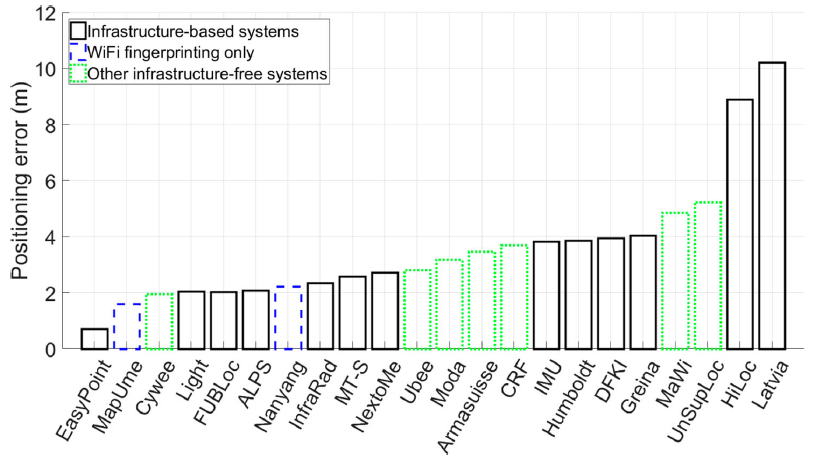
\includegraphics[scale=0.6]{figures/Competition.png}
  \caption{Performance de la précision du fingerprint lors de la compétition Microsoft IPSN 2014 competition \cite{CP_RSS}}
  \label{fig:Competition} %% NOTE: always label *after* caption!
 \end{center}
\end{figure}

Cela permet de mettre en évidence les précisions qui sont obtenues. Les algorithmes qui seront étudiés sont : Weighted K-nearest neighbours (W-KNN), Naïve Bayes Figure \ref{fig:PerfAccu}. Tous les mesures et tests sont basés sur le RSS du WIFI. 

\begin{figure}[htp]
 \begin{center}
  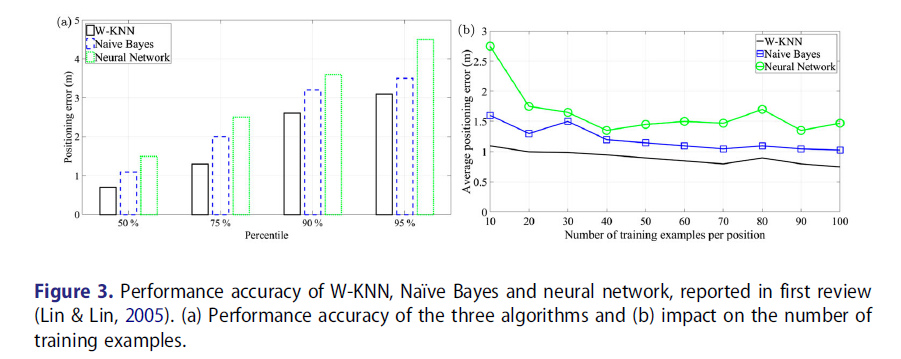
\includegraphics[scale=1]{figures/PerfAccu.png}
  \caption{Performance de la précision de W-KNN, Naïve Bayes et réseau de neurones, mais aussi l'impacte du nombre de données d'entrainement\cite{CP_RSS}}
  \label{fig:PerfAccu} %% NOTE: always label *after* caption!
 \end{center}
\end{figure}

Les mesures ont été effectuées de trois manières différentes (dans un corridor, sur un étage, sur trois étages - voir dans le document  \cite{CP_RSS}). En résumé, la synthèse des trois solutions suggère que, avec uniquement la mesure métrique WiFi RSS, de nombreux algorithmes complexes risquent de ne pas être aussi performants que des algorithmes plus simples. Malgré sa simplicité, W-KNN a excellé dans la plupart des analyses de "fingerprinting". Il convient de noter que le système MapUme, deuxième sur vingt-deux concurrents du concours Microsoft IPSN 2014, utilisait également W-KNN comme principal algorithme. Cependant, l'approche Naïve Bayes améliore sa précision lorsque le nombre d'entrainements est élevé, ce qui indique qu'au-delà du WiFi RSS, des informations supplémentaires seront nécessaires pour améliorer davantage les performances du "fingerprinting".

Une chose qui est également importante c'est la confiance qu'il y a dans un algorithme. Pour cela, cet article a utilisé "conformal prediction (CP)" afin de donner un indice de confiance. Plus la confiance est souhaité, plus il est nécessaire d'avoir de jeu de données. Les avantages d'utiliser l'indice de confiance sont les suivants:

\begin{enumerate}
 \item Chaque prédiction est associée à un indice de confiance et permet de dire combien la prédiction est correcte. 
 \item La prédiction produite par CP est statistiquement correcte sous les paramètres qui ont été choisis dans la phase on-line.
 \item le niveau de confiance peut être ajusté pour produire un ensemble de prédiction plus grand ou plus petit.
\end{enumerate}

Afin de valider leur algorithme, ils ont utilisé trois bancs de test Figure \ref{fig:TestBed}. 

\begin{enumerate}
 \item Royal Holloway : Données récoltées manuellement dans un office standard avec un smartphone
 \item Cambridge : Données récoltées automatiquement par un robot dans un environnement assez idéal.
 \item UJIIndoorLoc : Utilise le dataset public qui couvre une grande surface intérieure basée sur trois bâtiments.
\end{enumerate}

\begin{figure}[htp]
 \begin{center}
  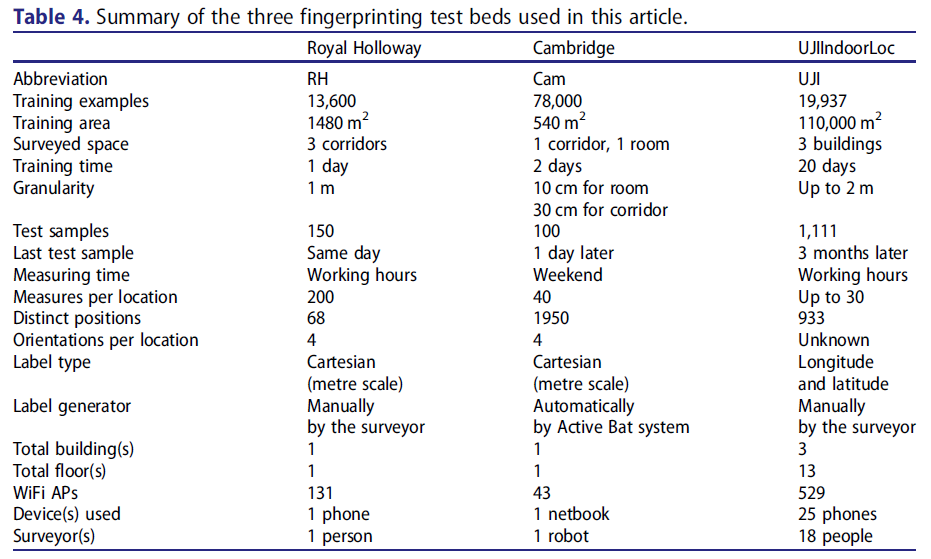
\includegraphics[scale=0.5]{figures/TestBed.png}
  \caption{Summary of the three fingerprinting test beds used in this article \cite{CP_RSS}}
  \label{fig:TestBed} %% NOTE: always label *after* caption!
 \end{center}
\end{figure}

Pour résumer cet article, il propose une nouvelle approche d'apprentissage basé sur la confiance d'un algorithme permettant d'estimer la position de l'utilisateur à l'intérieur avec la force du signal WiFi. Il introduit une mesure de confiance, non seulement utile pour refléter l'incertitude des prédictions de positionnement, mais également capable d'ajuster la taille de l'ensemble de prédictions en conséquence. 

Il a été montré empiriquement que la précision de positionnement était d’environ 2,4 m / probabilité de 75\% avec un banc d’essai normal, environ 70 cm / probabilité de 75\% avec un banc d’essai idéal et d’environ 8,8 m / probabilité de 75\% avec un banc d’essai difficile. 

Ces résultats ont surpassé les algorithmes de Machine Learning sans indice de confiance mis à l'essai sur les mêmes bancs d'essai jusqu'à 20\% plus précis. Si l'on ne tient pas compte de CP, l'algorithme W-KNN est un peu meilleur que Naïve Bayes. 

Les approches présentées dans cet article ne nécessitent pas de carte du bâtiment. Cela pourrait être utile de les avoir afin d'avoir des informations supplémentaires pour supprimer les mauvaises prédictions comme par exemple une personne qui marche dans un mur alors qu'elle est dans le couloir.

\section{Choix et conclusion}
Le choix de l'algorithme suite à l'analyse de l'état de l'art est une tâche difficile. Il est important de garder en tête l'application finale pour laquelle le système sera utilisé, c'est-à-dire, pour faire du positionnement intérieur.

En premier lieu, il est nécessaire de choisir entre un apprentissage par classification ou par régression. Il est clair que pour une utilisation finale un algorithme traitant de la régression comme SVM serait le mieux adapté. Ceci afin d'entrainer le système avec peu de positions et d'estimer les autres positions.

Cependant, il n'est pas vraiment réaliste de démarrer directement avec une technique pareil sans même savoir si les données disponibles sont exploitables. C'est pourquoi la décision a été de démarrer avec un algorithme de classification dans l'optique d'améliorer le système avec un algorithme de régression.

Suite, à l'étude des documents existants, il aurait été possible de sélectionner l'algorithme KNN qui a donnée dans la plupart des cas de bons résultats. Mon choix c'est dirigé vers l'algorithme SVM qui est également bien classé. Ce choix a été fait en grande partie, car il est également cité pour la régression en tant que SVR alors que KNN est uniquement cité pour de la classification. 

%\begin{enumerate}
% \item fgfd
% \item gdgfd
%\end{enumerate}


%\begin{figure}[H]
% \begin{center}
%  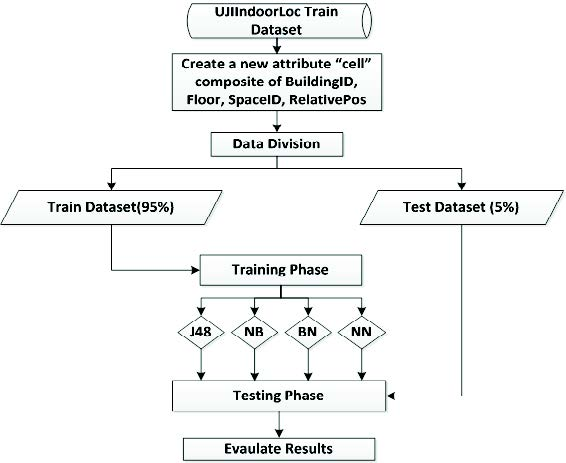
\includegraphics[scale=1]{figures/newattribute.jpg}
%  \caption{The new attribute “cell” construction phase}
%  \label{fig:newAttribute} %% NOTE: always label *after* caption!
% \end{center}
%\end{figure}

%\todo{Compléter cette partie qui semble importante}



% following structure:
%	000 => 099 abstract, acknoledgements,...
%	100 => 899 content
%	900 => 999 annexes, ...


%----------------------------------------------------------------------------------------
%	Bibliography
%----------------------------------------------------------------------------------------

%% prints every entry of the bib file -- useful in a state where is no cite
\appendix
\nocite{*}
\printbibliography

%----------------------------------------------------------------------------------------
%	Appendix
%----------------------------------------------------------------------------------------
%% add possible appendix
%\appendix
%\addpart*{Appendix}
%\chapter{Planning}
\begin{figure}[htp]
	\begin{center}
		\includegraphics[width=1\textwidth, angle=90]{../figures/pictures/000-planning.png}
		\caption[Planning]{Planning}
		\label{fig:planning} %% NOTE: always label *after* caption!
	\end{center}
\end{figure}





%----------------------------------------------------------------------------------------
%	\end{document}
%----------------------------------------------------------------------------------------
\end{document}
